
\chapter{Medição do volume de uma  moeda -- Propagação de incerteza}
\label{chap:volume}
\vspace{-0.7cm}

\section{Introdução}

Neste experimento determinaremos o volume de uma ou mais moedas.
Planeje o experimento antes de começar a realizar as medidas. Pense em quais métodos poderiam ser utilizados para se medir um volume, em quais medidas deveriam ser realizadas para esses m\'etodos e quais instrumentos seriam mais adequados para tal finalidade.


O volume pode ser determinado a partir das dimensões da moeda. Qual é a  expressão matemática do volume a partir dessas dimensões?

Se voc\^e conhecesse a massa e a densidade volumétrica de massa do material utilizado na fabricação da moeda, como você poderia determinar o seu volume ?

Se voc\^e tivesse  um recipiente com  água, como poderia determinar o volume de uma moeda imersa nesse líquido?

Avançando para a análise dos dados, como  estimar as incertezas das medidas diretas? Como são calculadas as incertezas das medidas indiretas?  Leia  as duas primeiras  seções do Capítulo~\ref{sec:medidasDir&Indir} (Conceitos Básicos para Análise de Dados).
Medindo a partir desses diferentes métodos, o que se espera da comparação dos seus  resultados?  Os valores deveriam ser compatíveis, considerando suas respectivas incertezas, independentemente do método utilizado?

Planejem seu experimento e comecem a fazer as anotações nos seus cadernos de laboratório. Para todos os experimentos que faremos nesse curso, cada um de vocês deve elaborar um pequeno texto no caderno para os seguintes tópicos: 

\begin{enumerate}
\item {\bf Introdução }
\item {\bf Procedimento Experimental}
\item {\bf Análise de Dados}
\item {\bf Discussão dos Resultados}
\end{enumerate}

%Agora que já planejou o experimento e já pensou sobre os resultados esperados,
%Separe os materiais necessários para o Experimento 2 (detalhes na Figura 1):
Separe os materiais necessários para o Experimento 2 (detalhes na Figura~\ref{fig:material}):

\begin{enumerate}
\item Moedas (sugerimos as de R\$ 0,50);
\item R\'egua;
\item Copo (que seja o mais pr\'oximo poss\'ivel da forma de um cilindro). Note que você pode simplificar e melhorar  a medição do volume deslocado, utilizando uma seringa descartável, que já vem  com uma escala volumétrica impressa.
\end{enumerate}


\begin{figure}[!hbt]
\centering
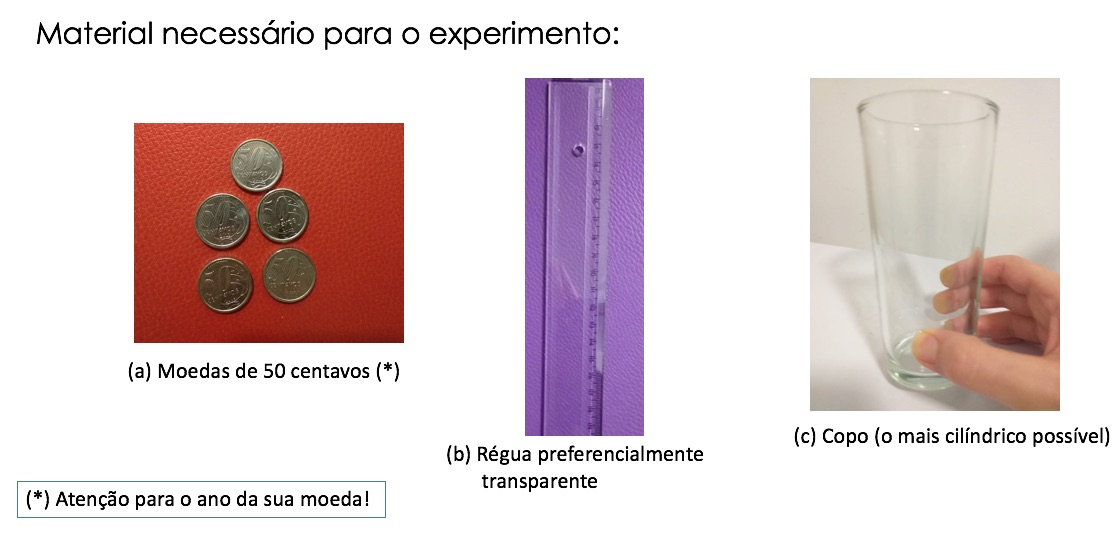
\includegraphics[height=0.28\paperheight]{Figuras_exp2/Foto1.jpg}
\caption{\label{fig:material} Material para o Experimento 2}
\end{figure}


\section{Procedimento experimental}
Antes de qualquer medida, se posicione de forma semelhante à sugerida na Figura~\ref{fig:observador}.

\begin{figure}[!hbt]
\centering
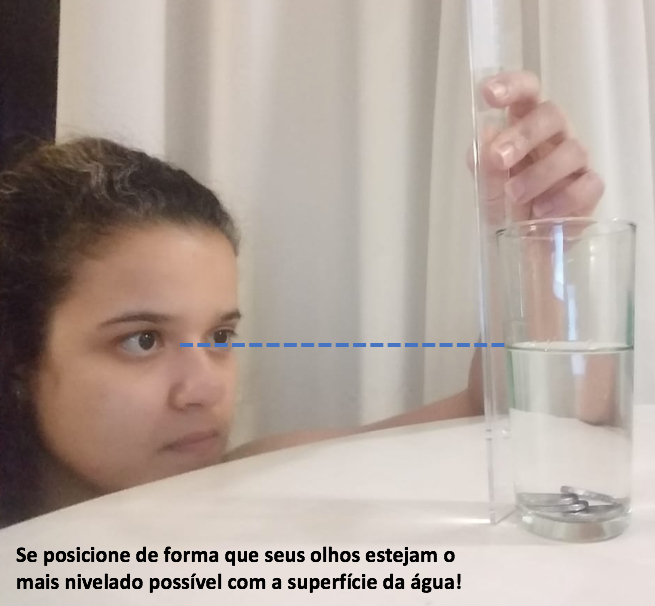
\includegraphics[height=0.28\paperheight]{Figuras_exp2/Foto2.jpg}
\caption{\label{fig:observador} Posicionamento do observador}
\end{figure}
\begin{enumerate}
\item {\bf A partir do volume de água deslocado}\\ 

Usando um copo cilíndrico parcialmente cheio d'água, introduza a(s) moeda(s) e estime o seu volume a partir do deslocamento do nível da coluna de água. No caso do copo, utilize uma régua para fazer essa medida a partir do registro dos níveis inicial e final.  Já com uma seringa descartável (Figura~\ref{fig:seringa}), o volume deslocado pode ser medido diretamente na seringa ao sugar a água, até que retorne ao mesmo nível da situação sem moeda(s), e lendo este volume na escala da própria seringa.  Dependendo do diâmetro do copo usado, avalie se o experimento deveria ser realizado com uma ou mais moedas de mesmo valor.

\begin{figure}[!hbt]
\centering
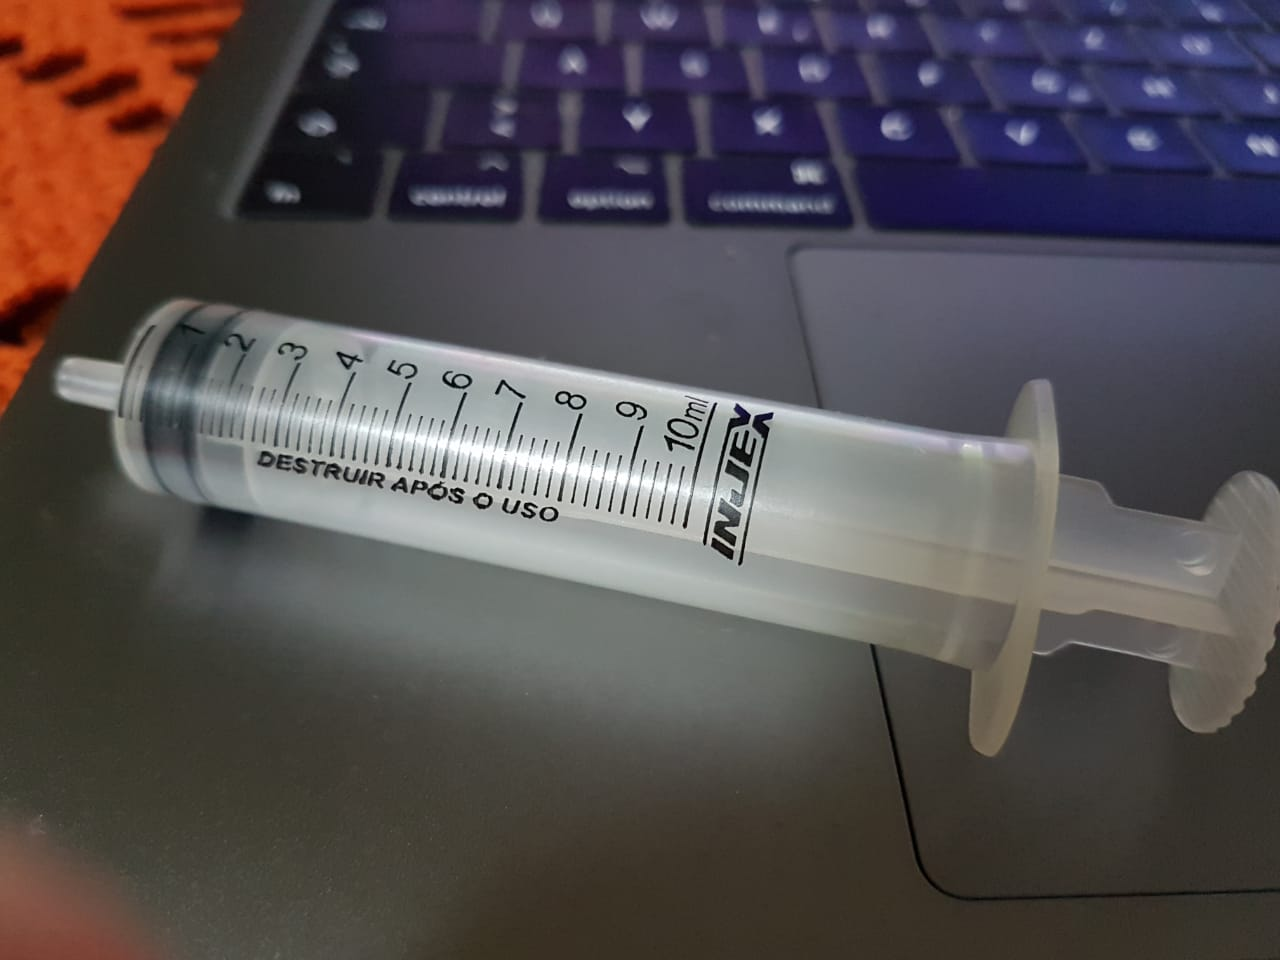
\includegraphics[height=0.18\paperheight]{Figuras_exp2/Foto3.jpeg}
\caption{\label{fig:seringa} Seringa}
\end{figure}


\item {\bf A partir da área da base da moeda  e de sua espessura}\\
Me\c ca  a espessura da moeda.  A área da base da moeda pode ser determinada  a partir da medição direta de seu diâmetro com uma régua ou a partir da medição de sua circunferência com o uso de um barbante e da régua.  Avalie qual procedimento é mais adequado.  A régua é o instrumento adequado para a determinação do 
di\^ametro da moeda? Nesse caso, tamb\'em avalie se o experimento deveria ser realizado com uma ou mais moedas do mesmo valor.

\item {\bf A partir da densidade volumétrica} \\
As moedas são fabricadas de forma padronizada  com relação às suas dimensões, massa e material.
Busque essas informações na Internet (página da Casa da Moeda). Fique atento que essas informações  podem variar de acordo com o ano de fabricação da moeda. A informação sobre o ano de fabricação consta na ``cara'' da mesma.
\end{enumerate}


\section{An\'alise de dados}
\begin{enumerate}
\item A partir dos valores  da espessura e do diâmetro ou circunferência da moeda,  medidos por você, calcule o volume da moeda utilizando uma das  fórmulas $V = \pi d^2 h/4  $ ($d =$ diâmetro e $h =$ espessura) ou $V=C^2 h/(4\pi)$ ($C =$ circunferência).

\item Sabendo que a densidade volumétrica do aço inoxid\'avel, dependendo da liga que o compõe, varia entre $7,8$ e $8,0$ g/cm$^3$, e utilizando o valor de massa padrão para a moeda utilizada, determine o seu volume e incerteza.
\item Organize em uma tabela os resultados obtidos para a determinação do volume da moeda com as respectivas incertezas para os três métodos realizados. Faça uma comparação entre os resultados obtidos. Leia  a segunda seção do Capítulo~\ref{sec:medidasDir&Indir} (Conceitos Básicos para Análise de Dados da Apostila). 
\end{enumerate}

\section{Discuss\~ao dos Resultados}
\begin{enumerate}
\item Qual foi a medição mais precisa? Justifique.
\item Considerando como referência o cálculo do volume da moeda a partir dos valores de suas dimensões encontrados na Internet, não os medidos por você, qual foi a medição mais exata? Justifique.
\item Justifique a vantagem de usar mais de uma moeda para o procedimento ``A partir do volume de água deslocado''.
\item   Os resultados encontrados são compatíveis entre si? Justifique. Esse resultado era esperado?
\item  Quais parâmetros contribuem mais fortemente para a incerteza do volume em cada um dos três métodos? Como essas incertezas poderiam ser diminuídas? Você sugere alguma modificação do procedimento experimental adotado?
\end{enumerate}



